\chapter{Optimierungen}
\label{chap:optimizer}
In diesem Kapitel wird beschrieben, was für Optimierungen für den Compiler implementiert wurden. Im Forth Cross-Compiler sind schon einige Peephole Optimierungen implementiert. In diesem Kapitel werden die neu implementierten Optimierungen mit dessen des Cross-Compilers verglichen und gezeigt wo noch bessere Optimierungsstrategien verwendet werden können.

\section{Peephole Optimierung}

Peephole Optimierungen ist eine Art von Optimierung, welche auf einer kleinen Sequenz von Instruktionen durchgeführt wird. Dieses Sequenz wird Peephole oder auch Window genannt. Die Peephole Optimierung verucht Sets von Instruktionen durch kürzere oder schnellere Instruktionen zu ersetzen.\cite{peepwiki} Peephole Optimierungen können die grösse des Codes um 15--40 Prozent verkleinern und sind heute in allen gängigen Compilern implementiert.\cite{peepdavidson} Zu den Peephole Optimierungen gehören unter anderen folgende Arten von Optimierungen:

\begin{itemize} 
	\item Constant Folding - Konstante Expressions auswerten
	\item Constant Propagation - Konstante Werte in Expressions substituieren
	\item Strength Reduction - Langsame Instruktionen mit äquivalenten schnellen Instruktionen ersetzen.
	\item Combine Operations - Mehrere Oprationen mit einer äquivalenten ersetzen
	\item Null Sequences - Unötige Operationen entfernen\cite{peepwiki}
\end{itemize}

\newpage

\subsection{Beispiele}

Folgend einige Peephole Optimierungs Beispiele anhand von Forth Code.

\subsubsection{Constant Propagation}
\label{constantprogationsection}

Folgende Instruktionen
%
\begin{verbatim}
1
2
swap
+
dup
\end{verbatim}
%
können durch:
%
\begin{verbatim}
2
2
\end{verbatim}
%
ersetzt werden. Die Instruktionen swap, + und dup können schon zur Kompilierzeit durchgeführt werden.
\subsubsection{Combine Operations}
Folgende zwei Instruktionen
%
\begin{verbatim}
rot
rot
\end{verbatim}
%
können durch
%
\begin{verbatim}
-rot
\end{verbatim}
%
ersetzt werden. Die zwei rot Instruktionen sind äquivalent zu einer -rot Instruktion. Oder die folgenden zwei Instruktionen
%
\begin{verbatim}
dup
drop
\end{verbatim}
%
können durch
%
\begin{verbatim}
nop
\end{verbatim}
%
ersetzt werden. Die zwei Instruktionen heben sich auf und können somit entfernt werden.

\newpage

\subsection{Optimierungen}

Für den Compiler wurden Prototypen mässig zwei Optimierungen in Java implementiert. Die erste Optimierung versucht benachbarte Instruktionen zu vereinfachen. Die zweite Optimierung ist eine einfache Constant Propagation. Die beiden Optimierungen werden in den nächsten Kapiteln genauer beschrieben. Der neue Optimizer wird in zwei Phasen durchgeführt:

\begin{figure}[H]
	\centering
		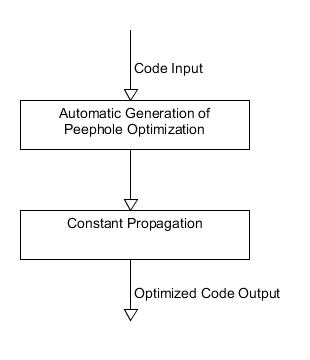
\includegraphics[scale=0.6]{optimizer/optimizer.png}
		\caption{Die zwei Phasen des Optimizers.}
		\captionsetup{margin=0cm,font={footnotesize}}
		\label{fig:optimizer}
\end{figure}

Im Cross-Compiler wurden unter anderem folgende Peephole Optimierungen schon implementiert.

\begin{enumerate}
  \item \verb!<lit> + ld, <lit> + st, <lit> + @!, and \verb!<lit> + \!! werden mit automatisch inkrementierenden Speicherzugriff Instruktionen ersetzt, wenn \verb!<lit>! sich zwischen \-4 und 3 befindet
  \item Folgende Stack Operationen: \\
				$swap, swap \rightarrow nop$\\
				$-rot, rot \rightarrow nop$\\
				$swap, + \rightarrow +$\\

\end{enumerate}

Für eine komplette Liste siehe "real time, object oriented with debugger" \cite{uforth}.

\newpage
\subsection{Automatische Generierung von Peephole Optimierungen}

Klassische Peephole Optimizer versuchen häufig einige Maschinenspezifische Patterns zu korrigieren. Der von Davidson und Fraser\cite{peepdavidson} beschriebene Algorithmus (PO) verwendet eine Machine Description, simuliert benachbarte Instruktionen und versucht diese mit äquivalenten, schnelleren Instruktionen zu ersetzen. Für den Forth Optimizer wurde ein Teil des PO objektorientiert implementiert.

\subsection{Constant Propagation}
Unter Constant Propagation versteht man, dass vorwärts substituieren von Konstanten im Code. Dies kann zur Folge haben, dass mehrere Instruktionen schon zur Kompilierzeit ausgewertet werden können, wie bei den Beispielen \ref{constantprogationsection} zu sehen ist.

\subsection{Resultate und Tests}
Die Resultate des Optimierers wurden mit verschiedenen Forth Funktionen getestet und die Resultate mit dem Peephole Optimizer des uForth Cross-Compilers verglichen. Der Source-Code zu den getesteten Funktionen befindet sich im Anhang.

\begin{table}[H]
\begin{center}
    \begin{tabular}{ | l | l | l | l | p{8cm} |}
    \hline
    \textbf{Funktion} & \textbf{Orig} & \textbf{Ref} & \textbf{Neu} & \textbf{Kommentar} \\ \hline
    \_Init & 126 & 112 & 119 & Die Referenzimplementierung produziert vor allem wegen der Speicherzugriffsoptimierung kürzeren Code. Constant Propagation, welche neu implementiert wurde, konnte keine durchgeführt werden. PO konnte Instruktionspaare finden, welche weg optimiert werden können.  \\ \hline
		\_Update & 8 & 8 & 4 & PO konnte zwei Instruktionspaare weg optimieren, welche von der Referenzimplementierung nicht optimiert werden. \\ \hline
		\_Hash & 65 & 60 & 60 & Die Referenzimplementierung produziert wieder wegen der Speicherzugriffsoptimierung weniger Code. PO konnte wieder Instruktionspaare finden, welche weg optimiert werden können. \\ \hline
		\_Propagation & 11 & 11 & 4 & Bei dieser Funktion konnte vor allem Constant Propagation durchgeführt werden. Die Referenzimplementierung führt keine Constant Propagation durch. \\ \hline
    \end{tabular}
		\caption{Resultate des neuen Optimizers verglichen mit dem Cross-Compiler Optimizer.}
		\label{tab:peepresults}
\end{center}
\end{table}
\newpage

Es hat sich herausgestellt, dass bei allen Beispielen die Constant Propagation nur wenig Code optimieren konnte. Dies ist vermutlich der Fall, weil konstante Ausdrücke schon vom Compiler optimiert werden und die implementierte Constant Propagation zu primitiv ist. Im nächsten Kapitel werden einige Erweiterungen vorgeschlagen, um diese effizienter zu gestalten.  

PO konnte Regeln finden, welche vom Forth-Cross Compiler noch nicht erkannt werden. Unter anderem folgende:\\ \\
%
$swap, swap \rightarrow nop$\\
$-rot, rot \rightarrow nop$\\
$rot, -rot \rightarrow nop$\\
$1, + \rightarrow 1+$\\
$swap, + \rightarrow +$\\
%

Diese Regeln könnten im Forth Cross-Compiler integriert werden. Im nächsten Kapitel werden Änderungen für den PO vorgeschlagen, damit dieser mehr mögliche Instruktionsketten erkennen könnte, welche vereinfacht werden können.

\subsection{Mögliche Erweiterungen}

Im Moment werden vom PO nur Insturktionen, welche einen Einfluss auf den Daten Stack haben simuliert. PO könnte erweitert werden, indem weitere Instruktionen auch simuliert werden. Eine weiter Möglichkeit wäre, der von Bansal und Aiken beschriebene Superoptimizer zu implementierten. Dieser Superoptimizer verwendet Bruteforce Optimierungen mittels tausenden von Regeln. Diese Regeln werden von Trainings Programmen inferiert und in einer Datenbank gespeichert.\cite{superoptimizer}

Die Constant Propagation könnte noch so erweitert werden, dass sie auch mit Branches umgehen kann. Somit könnten unnötige If-Statements, sowie Schleifen entfernt werden. Um dies zu implementieren müsste der Code zuerst in eine static single assignemt form (SSA) transformiert werden.\cite{ssa} Es wäre somit aber keine Peephole Optimierung mehr.